\documentclass{article}[10pt]
\usepackage{relsize}
\usepackage{amsthm}
\usepackage{amsmath}
\usepackage{amssymb}
\usepackage{todonotes}
\usepackage{cite}
% \input{../Latex/MarksFront10}

\textwidth=6.5in
\hoffset-.75in
\textheight=9in
\voffset-.5in

\begin{document}

\title{Mini Quiz \\  Professor Marks \\ ELC 5354}

\date{\today}

\maketitle





\begin{itemize}
\item The exam is due on midnight May 10, 2015.
\item Your solution is to be written in \LaTeX. The \LaTeX
  file and the corresponding pdf file is to be emailed to \verb"Robert_Marks@Baylor.edu" by the deadline.
\item Show your work.
\item No human resource will be consulted in the execution of the exam.
\end{itemize}



\section{Exam}

\begin{enumerate}




\item Let the second characteristic function of a random variable $X$ be
  $$ \Psi_X (u ) = a + bu + cu^2 + u^{10} .$$
  Given the mean, $\mu$, and the variance, $\sigma^2$, what are the values of $a$, $b$, and $c$?



\item Consider the stochastic process
  $$X(t)= \cos (2 \pi t + \Theta  )$$
  where $\Theta$ is  a random variable uniform on $(-\pi, \pi)$.
  \begin{enumerate}
  \item Is $X(t)$ WSS?
    \begin{enumerate}
    \item If not, why?
    \item If so, what is the average power of $X(t)$ on the interval $0\leq u \leq 1.5$? On $1.5\leq u \leq 27$?
    \end{enumerate}
  \item Is $X(t)$ stationary in the strict sense?
  \item If $X(t)$ mean ergodic?
  \end{enumerate}
  Explain each answer.


\item  We roll a die.  If five dots show, we flip on an oscillator that generates $X(t) = \sin (2 \pi t)$ volts.  Otherwise, we turn on a one volt DC (constant) power supply and get $X(t)=1$.
  \begin{enumerate}
  \item  What is the expected value of $X(t)$ at $t=1$?
  \item  What is the variance of $X(t)$ at $t=1$?
  \item   What is the cumulative distribution, $F_X (x)$, of $X(t)$ at $t=1$?
  \item  Are there any values of $t$ where $X(t)$ is deterministic?
    % \item  Is $X(t)$ ergodic?\footnote{No math is required. Just an explanation.}
  \end{enumerate}

\item  Let $X(t)$ be the Poisson counting process with parameter $\lambda$.
  \begin{enumerate}
  \item Let
    $$ Y(t) = X(t) - \lambda t .$$
    Evaluate the mean and autocorrelation of $Y(t)$.
  \item Let
    $$Z(t) = \frac{dY(t)}{dt}.$$
    Evaluate the mean and autocorrelation of $Z(t)$.
  \item Fill in the following table indicating the properties of $X(t)$, $Y(t)$ and $Z(t)$. Each block should contain either a `yes' or a `no'.

    \begin{tabular}{|r||c|c|c|}\hline
      $\downarrow$ Property $|$ Process $\rightarrow$                     & $X(t)$    &  $Y(t)$   & $Z(t)$    \\ \hline
      Zero Mean                                                           &           &           &           \\ \hline
      Wide Sense Stationary                                               &           &           &           \\ \hline
      White Noise                                                         &           &           &           \\ \hline
      Gaussian White Noise                                                &           &           &           \\ \hline
    \end{tabular}
  \end{enumerate}




\item The autocorrelation of a zero mean voltage noise source, $V(t)$, is
  $$ R_V (\tau ) = 10 \; \exp(-|\tau|)\mbox{ volt}^2.$$
  Time $t$ is measured in seconds and frequency $f$ in Hertz. We are going to analyze this voltage source in three different scenarios.
  \begin{enumerate}
  \item $V(t)$ is applied across a 5 ohm resister. What is the average power dissipated by the resister?


  \item  The voltage $V(t)$ is applied across a series connection of a 2 ohm resistance and a one farad capacitor. Call the voltage across the resister $U(t)$.
    \begin{enumerate}
    \item What is the power spectral density of $U(t)$?

    \item What is the autocorrelation of the noise across the resister?

    \item What is the average power dissipated by the resister?


    \end{enumerate}
  \item The voltage $V(t)$ is passed through a low pass voltage filter that discards all frequency components higher that 4 Hertz and keeps the rest. The voltage at the filter output is applied across a four ohm resister. What power is dissipated by the resister?
  \end{enumerate}


\end{enumerate}

\section{Old Quiz}

Here is the previous miniQuiz. If you received a perfect score of 4, your points will be doubled. If not, you can rework the problem. Grading is binary. Either 4 points for a correct solution or zero.

\begin{enumerate}
\item
  Let $X$ and $Y$ be i.i.d. random variables distributed as
  $$ f_X(x) = f_X(x) = e^{-x} \mu (x)$$
  Find $f_Z (x)$ if
  \begin{enumerate}
  \item $Z=-X-Y$.
  \item $Z=\frac{X}{Y}$
  \end{enumerate}
\end{enumerate}

\begin{figure}
  \centering
  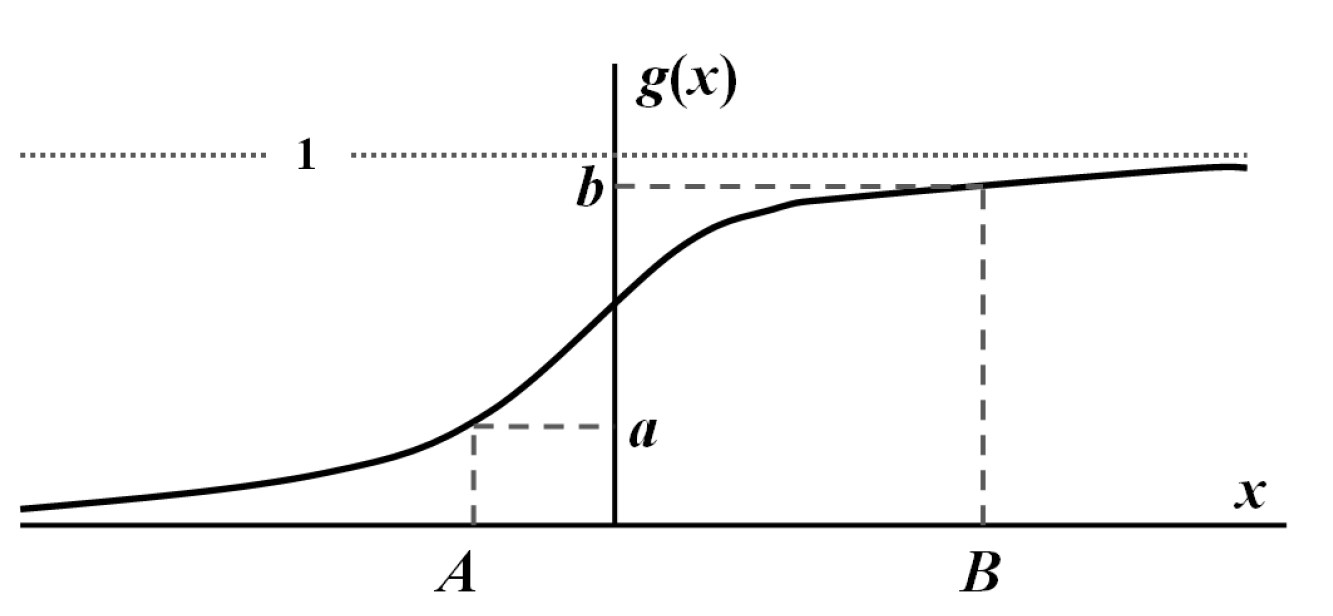
\includegraphics[width=3in]{pics/PROB.png}
  \caption{Figure for Problem~\ref{PNutButt01}.}
  \label{PNutButt03}
\end{figure}

\section{For Fun}

I was going to assign this problem, but decided not to. It's here only for fun.

\begin{enumerate}
\item
  \label{PNutButt01}

  You are given two envelopes. Inside each is a slip of paper with two numbers
  written on them. The two numbers are not the same. The way the numbers
  are chosen is unknown. You chose one of the envelopes at random. You open
  it and look at the number. You must make a choice. Either the number you
  hold is the largest number or the number in unopened envelope is and you
  have to make a decision.
  If you choose the largest of the two numbers, you get a million dollars.
  If it isn't, you get nothing.
  At first, it looks like anything you do won't help you win beyond a
  50-50 chance. But is this true? Can you always make a decision that gives you
  a strictly better than a 50-50 chance of winning? Consider the following algorithm.
  Here are the steps.
  \begin{enumerate}
  \item Choose any squashing function $g(x)$ that maps $(-\infty, \infty)$ to the interval (0,1). As shown in Figure~\ref{PNutButt03}, the function
    must be strictly increasing but is otherwise arbitrary. Examples are the sigmoid
    $$F (x)=\frac{1}{1+e^{-\alpha x}} ; \alpha >0$$
    or
    $$ g(x) = \frac{1}{2} + \frac{1}{\pi} \arctan \left( \frac{x-\mu}{\sigma} \right) ; \sigma >0, \mu \mbox{ real}. $$
  \item Choose an envelope at random and open it. The contents is the number $C$. Let $c=g(C)$. Note that $0 <c <1$.
  \item Use a random number generator, like on MATLAB, to produce a uniform random variable $X$ between zero and one. This random number tells you what to do.
    \begin{enumerate}
    \item If $X<c$, then keep $C$. Do not open the other envelope.
    \item Otherwise, open the other envelope.
    \end{enumerate}
  \end{enumerate}
  Here is a proof that this will result in a win with a chance greater that 50-50.
  \begin{enumerate}
  \item Let the two envelopes be marked $\mathbb{A}$ and $\mathbb{B}$. Assume with no loss of generality, that
    envelope $\mathbb{B}$ contains the biggest number so that $B > A$. Thus, since $g(x)$ is strictly increasing, $g(B) > g(A)$. Thus
    \begin{equation}
      b>a
      \label{PNutButt02}
    \end{equation}
    where $b=g(B)$ and $a= g(A)$.
  \item Let $p$ denote your probability of success. Since choosing envelopes $\mathbb{A}$ or $\mathbb{B}$ are mutually exclusive events,
    \begin{eqnarray}
      p &=& \Pr \left[ (\mbox{choose } \mathbb{B}\mbox{ and don't switch envelopes) OR (choose } \mathbb{A} \mbox{ and switch envelopes}) \right] \nonumber \\
        &=&  \Pr  \left( X<b \mbox{ and you first chose envelope $\mathbb{B}$.} \right) +
            \Pr \left( X>a \mbox{ and you first chose envelope $\mathbb{A}$} \right). \nonumber
    \end{eqnarray}
  \item Given that each envelope is chosen with a 50-50 chance and $X$ is uniform, it follows that
    \begin{eqnarray}
      p &=& \frac{1}{2} \; b + \frac{1}{2}(1-a)   \nonumber \\
        &=& \frac{1}{2} + \frac{1}{2} (b-a)  \nonumber
    \end{eqnarray}
    From (\ref{PNutButt02}), $b-a>0$ which means that your chances of winning are greater than 50-50. That is
    $$p > \frac{1}{2}.$$
  \end{enumerate}

  {\bf Is this analysis correct?}

  \begin{enumerate}
  \item If so, illustrate convincingly using Monte Carlo simulation.
  \item If not, identify the location of the faulty reasoning in the proof.
  \end{enumerate}
\end{enumerate}
\end{document}
